\section*{Chapter 0: Introduction}
\addcontentsline{toc}{section}{Chapter 0: Introduction}

\subsection*{0.4}

If A has a elements and B has b elements, how many elements are in A $\times$ B? Explain your answer.

\paragraph{Solution.}
We claim that
\[
|A \times B| = ab.
\]
Indeed, by definition,
\[
A \times B = \{(x,y) \mid x \in A,\ y \in B\}.
\]
For each fixed element $x \in A$, there are exactly $b$ possible choices for the second coordinate $y \in B$. Hence each $x$ contributes exactly $b$ ordered pairs to $A \times B$. Since there are $a$ possible choices for $x$, the multiplication principle gives
\[
|A \times B| = a \cdot b = ab.
\]
Therefore, the Cartesian product $A \times B$ has exactly $ab$ elements.

\paragraph{案：} 根据笛卡尔积的定义，这个问题可以分三步来理解。首先，$A \times B$ 中的一个元素是一个有序对，它由两个集合中各取一个元素构成。其次，固定 $A$ 中的一个元素，它都可以与 $B$ 中
  的每一个元素配对，因此恰好产生 $b$ 个有序对。最后，由于 $A$ 中一共有 $a$ 个元素，所以这样的有序对总数为 $a \cdot b = ab$。


\subsection*{0.7}

For each part, give a relation that satisfies the condition.

\begin{enumerate}[label=(\alph*), leftmargin=2.5em]

\item Reflexive and symmetric but not transitive

\item Reflexive and transitive but not symmetric

\item Symmetric and transitive but not reflexive

\end{enumerate}

\paragraph{Solution.}
We give explicit examples.

\begin{enumerate}[label=(\alph*), leftmargin=2.5em]

\item Let $X = \{1,2,3\}$, and define a relation $R$ on $X$ by
\[
xRy \iff |x-y| \leq 1.
\]
Then $R$ is reflexive because $|x-x|=0 \leq 1$ for every $x \in X$. It is symmetric because if $|x-y| \leq 1$, then also $|y-x| \leq 1$. However, $R$ is not transitive: we have $1R2$ and $2R3$, but $1 \not R 3$ because $|1-3|=2>1$.

\item Let $X = \{1,2\}$, and define
\[
R=\{(1,1),(1,2),(2,2)\}.
\]
This relation is reflexive because $(1,1)$ and $(2,2)$ both belong to $R$. It is transitive because the only possible compositions of pairs in $R$ again produce pairs already in $R$. But $R$ is not symmetric, since $(1,2)\in R$ whereas $(2,1)\notin R$.

\item Let $X = \{1,2\}$, and define
\[
R=\{(1,1)\}.
\]
Then $R$ is symmetric because the reverse of $(1,1)$ is again $(1,1)$. It is transitive because composing $(1,1)$ with itself yields $(1,1)$, which is still in $R$. However, $R$ is not reflexive on $X$, since reflexivity would require both $(1,1)$ and $(2,2)$ to lie in $R$, but $(2,2)\notin R$.

\end{enumerate}

\paragraph{案：}  可以把关系看成定义在某个顶点集上的一组有向边。这样一来，自反性对应于每个顶点都有一个自环；对称性对应于若存在边 $x \to y$，则也必须存在边 $y \to x$；传递性对应于只要存在
  路径 $x \to y \to z$，就必须再有一条边 $x \to z$。因此，从图的视角来看，这道题实际上是在构造满足若干边性质、但不满足另一些边性质的小型有向图。这个视角对于寻找反例和构造例子都很有帮助。

\subsection*{0.9}

Write a formal description of the following graph.

\begin{figure}[h]

\centering

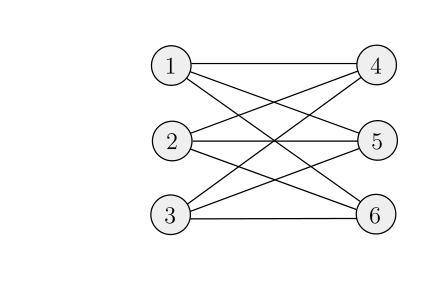
\includegraphics[width=0.42\textwidth]{chapters/assets/exercise_0_9_graph.png}

\caption*{Graph from Exercise 0.9}

\end{figure}

\paragraph{Solution.}
This graph is the complete bipartite graph $K_{3,3}$. A formal description is
\[
G=(V,E),
\]
where
\[
V=\{1,2,3,4,5,6\},
\]
and
\[
E=\bigl\{\{i,j\}\mid i\in\{1,2,3\},\ j\in\{4,5,6\}\bigr\}.
\]
Equivalently, one may list the edge set explicitly as
\[
E=\{\{1,4\},\{1,5\},\{1,6\},\{2,4\},\{2,5\},\{2,6\},\{3,4\},\{3,5\},\{3,6\}\}.
\]
Hence the graph has bipartition $\{1,2,3\}$ and $\{4,5,6\}$, and every vertex in the first part is adjacent to every vertex in the second part.


\subsection*{0.10}

Show that every graph with two or more nodes contains two nodes that have equal degrees.


\subsection*{0.11}

Find the error in the following proof that all horses are the same color. C LAIM : In any set of h horses, all horses are the same color. PROOF : By induction on h.

Basis: For h = 1. In any set containing just one horse, all horses clearly are the same color.

Induction step: For k $\ge$ 1, assume that the claim is true for h = k and prove that it is true for h = k + 1. Take any set H of k + 1 horses. We show that all the horses in this set are the same color. Remove one horse from this set to obtain the set H1 with just k horses. By the induction hypothesis, all the horses in H1 are the same color. Now replace the removed horse and remove a different one to obtain the set H2 . By the same argument, all the horses in H2 are the same color. Therefore, all the horses in H must be the same color, and the proof is complete.


\subsection*{0.13}

Find the error in the following proof that 2 = 1. Consider the equation a = b. Multiply both sides by a to obtain a2 = ab. Subtract b2 from both sides to get a2 - b2 = ab - b2 . Now factor each side, (a + b)(a - b) = b(a - b), and divide each side by (a - b) to get a + b = b. Finally, let a and b equal 1, which shows that 2 = 1.


\clearpage
